% Chapter Chapter 8 For Reproducible Research in R and RStudio
% Christopher Gandrud
% Created: 16/07/2012 05:45:03 pm CEST
% Updated: 11 October 2012




\chapter{Statistical Modelling and knitr}\label{StatsModel}

To make your research reproducible, you should directly connect your presentation documents to the source code you used to analyse the data you have collected. We primarily tie our statistical analyses and presentation documents together with {\emph{knitr}}. In Chapter \ref{GettingStartedRKnitr} we learned basic {\emph{knitr}} syntax. In this chapter we will look at {\emph{knitr}} syntax in much more detail, particularly code chunk options. You will also learn how to include code chunks as separate blocks from the text of your LaTeX and Markdown presentation documents. You will also learn to include code chunks in-line with your presentation documents' text.

The goal of this and the next two chapters is to show you how to tie your analyses into your presentation documents so closely that every time the documents are compiled they actually reproduce your analysis and present the results.

Please see the next part of this book, Part IV, for details on how to create the LaTeX and Markdown documents that can include {\emph{knitr}} code chunks.

\todo[inline]{Much of this chapter is incomplete.}

\section{Incorporating analyses into the markup}

\subsection{Full code chunks}

\subsubsection{LaTeX}

\subsubsection{Markdown}

\subsection{Showing code \& results inline}

Sometimes we want to have some R code or output to show up in the text of our documents. We may want to include stylized code in our text when we discuss how we did an analysis. We may want to report the mean of some variable in our text.

\subsubsection{LaTeX}

\paragraph{Inline static code}

If we just want to include a code snippet in out text we can simply use the LaTeX command  \texttt{\textbackslash{}tt}. This sets our text to `typewriter' font, the standard font for inline code in LaTeX (I use it in this book, as you have probably noticed).

\paragraph{Inline dynamic code}

If we want to dynamically show the results of some R code in our text we can use the  \texttt{\textbackslash Sexpr} command. This is a pseudo LaTeX command. Its structure is more like a LaTeX command's structure than \texttt{knitr} in that we enclose our R code in curly brackets (\texttt{\{\}}) rather than the usual \texttt{\textless\textless\textgreater\textgreater= . . . @} syntax for code chunks.

For example, imagine that we wanted to include the mean--591--in the text of our document. The {\emph{rivers}} numeric vector, loaded by default in R, has the length of 141 major rivers recorded in miles. We can simply use the {\tt{mean}} command to find the mean and the {\tt{round}} command to round it to the nearest whole number:

\begin{knitrout}
\definecolor{shadecolor}{rgb}{0.969, 0.969, 0.969}\color{fgcolor}\begin{kframe}
\begin{alltt}
\hlfunctioncall{round}(\hlfunctioncall{mean}(rivers), digits = 0)
\end{alltt}
\begin{verbatim}
## [1] 591
\end{verbatim}
\end{kframe}
\end{knitrout}


\noindent To have just the output show up inline with the text of our document we would type something like:

\begin{knitrout}
\definecolor{shadecolor}{rgb}{0.969, 0.969, 0.969}\color{fgcolor}\begin{kframe}
\begin{alltt}
The mean length of 141 major rivers in North America
is \textbackslash{}Sexpr\{\hlfunctioncall{round}(\hlfunctioncall{mean}(rivers), digits = 0)\} miles. 
\end{alltt}
\end{kframe}
\end{knitrout}


\noindent This will produce the sentence:

\begin{quote}
    The mean length of 141 major rivers in North America is 591 miles. 
\end{quote}

\subsubsection{Markdown}

\paragraph{Inline static code}

To include static code inline in an R Markdown (and regular Markdown) document we enclose the code in single backticks (\` \`). For example typing

\begin{knitrout}
\definecolor{shadecolor}{rgb}{0.969, 0.969, 0.969}\color{fgcolor}\begin{kframe}
\begin{alltt}
This is example R code: `MeanRiver <- \hlfunctioncall{mean}(rivers)`.
\end{alltt}
\end{kframe}
\end{knitrout}


\noindent produces:\footnote{The exact look of the text depends on the CSS\index{CSS} style file you are using.}


\includegraphics[scale = 0.6]{/git_repositories/Rep-Res-Book/Source/Children/Chapter8/images8/MeanRiverMarkdown.png}

\paragraph{Inline dynamic code}

Including dynamic code in the body of your R Markdown text is similar to including static code. The only difference is that we put the letter \texttt{r} after the first single backtick. For example:

\begin{knitrout}
\definecolor{shadecolor}{rgb}{0.969, 0.969, 0.969}\color{fgcolor}\begin{kframe}
\begin{alltt}
`r \hlfunctioncall{mean}(rivers)`
\end{alltt}
\end{kframe}
\end{knitrout}


\noindent will include the mean value of the {\emph{rivers}} vector in the text of your Markdown document.

\subsection{Sourcing R code from another file}

There are a number of reasons that you might want to have your R source code located in a separate file from your markup even if you plan to compile them together with {\emph{knitr}}.

First, it can be unwieldy to edit both your markup and long R source code chunks in the same document, even with RStudio's handy {\emph{knitr}} code collapsing and chunk management options. There are just too many things going on in one document.

Second, you may want to use the same code in multiple documents--an article and presentation for example. It is nice to not have to copy and paste the same code into multiple places, but have multiple documents link to the same source code. Plus if you make changes to the source code, these changes will automatically be made across all of your presentation documents. You don't need to make the same changes multiple times.

Third, other researchers trying to replicate your work might only be interested in specific parts of your analysis. If you have the analysis broken into separate and clearly labeled files it is easier for these
researchers to find the specific bits of code that they are interested compared to digging through long markup files.

\subsubsection{Source from a local file}

Usually in the early stages of research you may want to source analysis iles located on your computer. Doing this is simple. The {\emph{knitr}} syntax is the same as above. The only change is that instead of writing all of our code in the chunk we save it to its own file and use the \texttt{source} command in \emph{base} R to access it. For example:

\subsubsection{Source from a non-secure URL (\texttt{http})}

Sourcing from your local computer is fine if you are working alone and do not want others to access your code. Once you start collaborating and generally wanting people to be able to replicate your code, you need to
use another method.\footnote{You can make the replication code accessible for download and either instruct others to change the working directory to the replication file or have them change the directory information as necessary. However, this usually just adds an extra complicating step that makes replication harder. It is also a   pain if you are collaborating and each author has to constantly change the directories.}

The simplest solution to these issues is to host the replication code in your Dropbox public folder. You can find the file's public URL the same way we did in Chapter 6. Now use the \texttt{source} command the same way as before. For example:

\subsubsection{Source from a secure URL (\texttt{https})}

If you are using GitHub\index{GitHub} or another service that uses secure URLs to host your analysis source code files the steps are generally the same, but you need to use the \texttt{source\_url} command in the {\emph{devtools}} package. For GitHub based source code we find the file's URL the same way we did in Chapter \ref{Storing}. Remember to use the URL for the {\emph{raw}} version of the file. I have a short script hosted on GitHub for creating a scatter plot from data in R's {\emph{cars}} data set. The script's shortened URL is \url{http://bit.ly/Ny1n6b}.\footnote{The original URL is at \url{https://raw.github.com/christophergandrud/christophergandrud.github.com/master/SourceCode/CarsScatterExample.R}. This is very long, so I shortened it using bitly (see \url{http://bitly.com}). You may notice that the shortened URL is not secure. However, it does link to original secure {\tt{https}} URL.} To run this code and create the scatter plot using {\tt{source\_url}} we simply type:

\begin{knitrout}
\definecolor{shadecolor}{rgb}{0.969, 0.969, 0.969}\color{fgcolor}\begin{kframe}
\begin{alltt}
\hlcomment{# Load library}
\hlfunctioncall{library}(devtools)

\hlcomment{# Create object to hold URL}
URL <- \hlstring{"http://bit.ly/Ny1n6b"}

\hlcomment{# Run the source code to create the scatter plot}
\hlfunctioncall{source_url}(URL)
\end{alltt}
\end{kframe}

{\centering 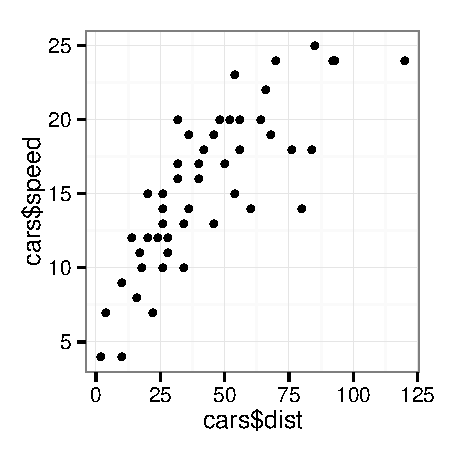
\includegraphics[width=\maxwidth]{figure/Ch8SourceURLExample} 

}


\end{knitrout}


\section{Saving output objects for future use}

\section{Literate Programming: Including highlighted syntax in the output}

\subsection{LaTeX}

\subsection{Markdown/HTML}

\section{Debugging}

